\section{Generazioni cellulari}
Nel corso degli anni, si sono susseguite diverse generazioni di tecnologie cellulari, che hanno apportato
notevoli cambiamenti alla loro architettura. Di seguito verranno presentati le principali caratteristiche
delle diverse generazioni cellulari, in modo tale da rendere di facile comprensione l'analisi dei meccanismi
di identificazione che verranno approfonditi nelle prossime sezioni.\\
Oltre ad elencare le principali caratteristiche di ogni generazione verranno analizzate nel dettaglio le specifiche  
dell'architettura di rete.
\begin{figure}[ht]
    \centering
    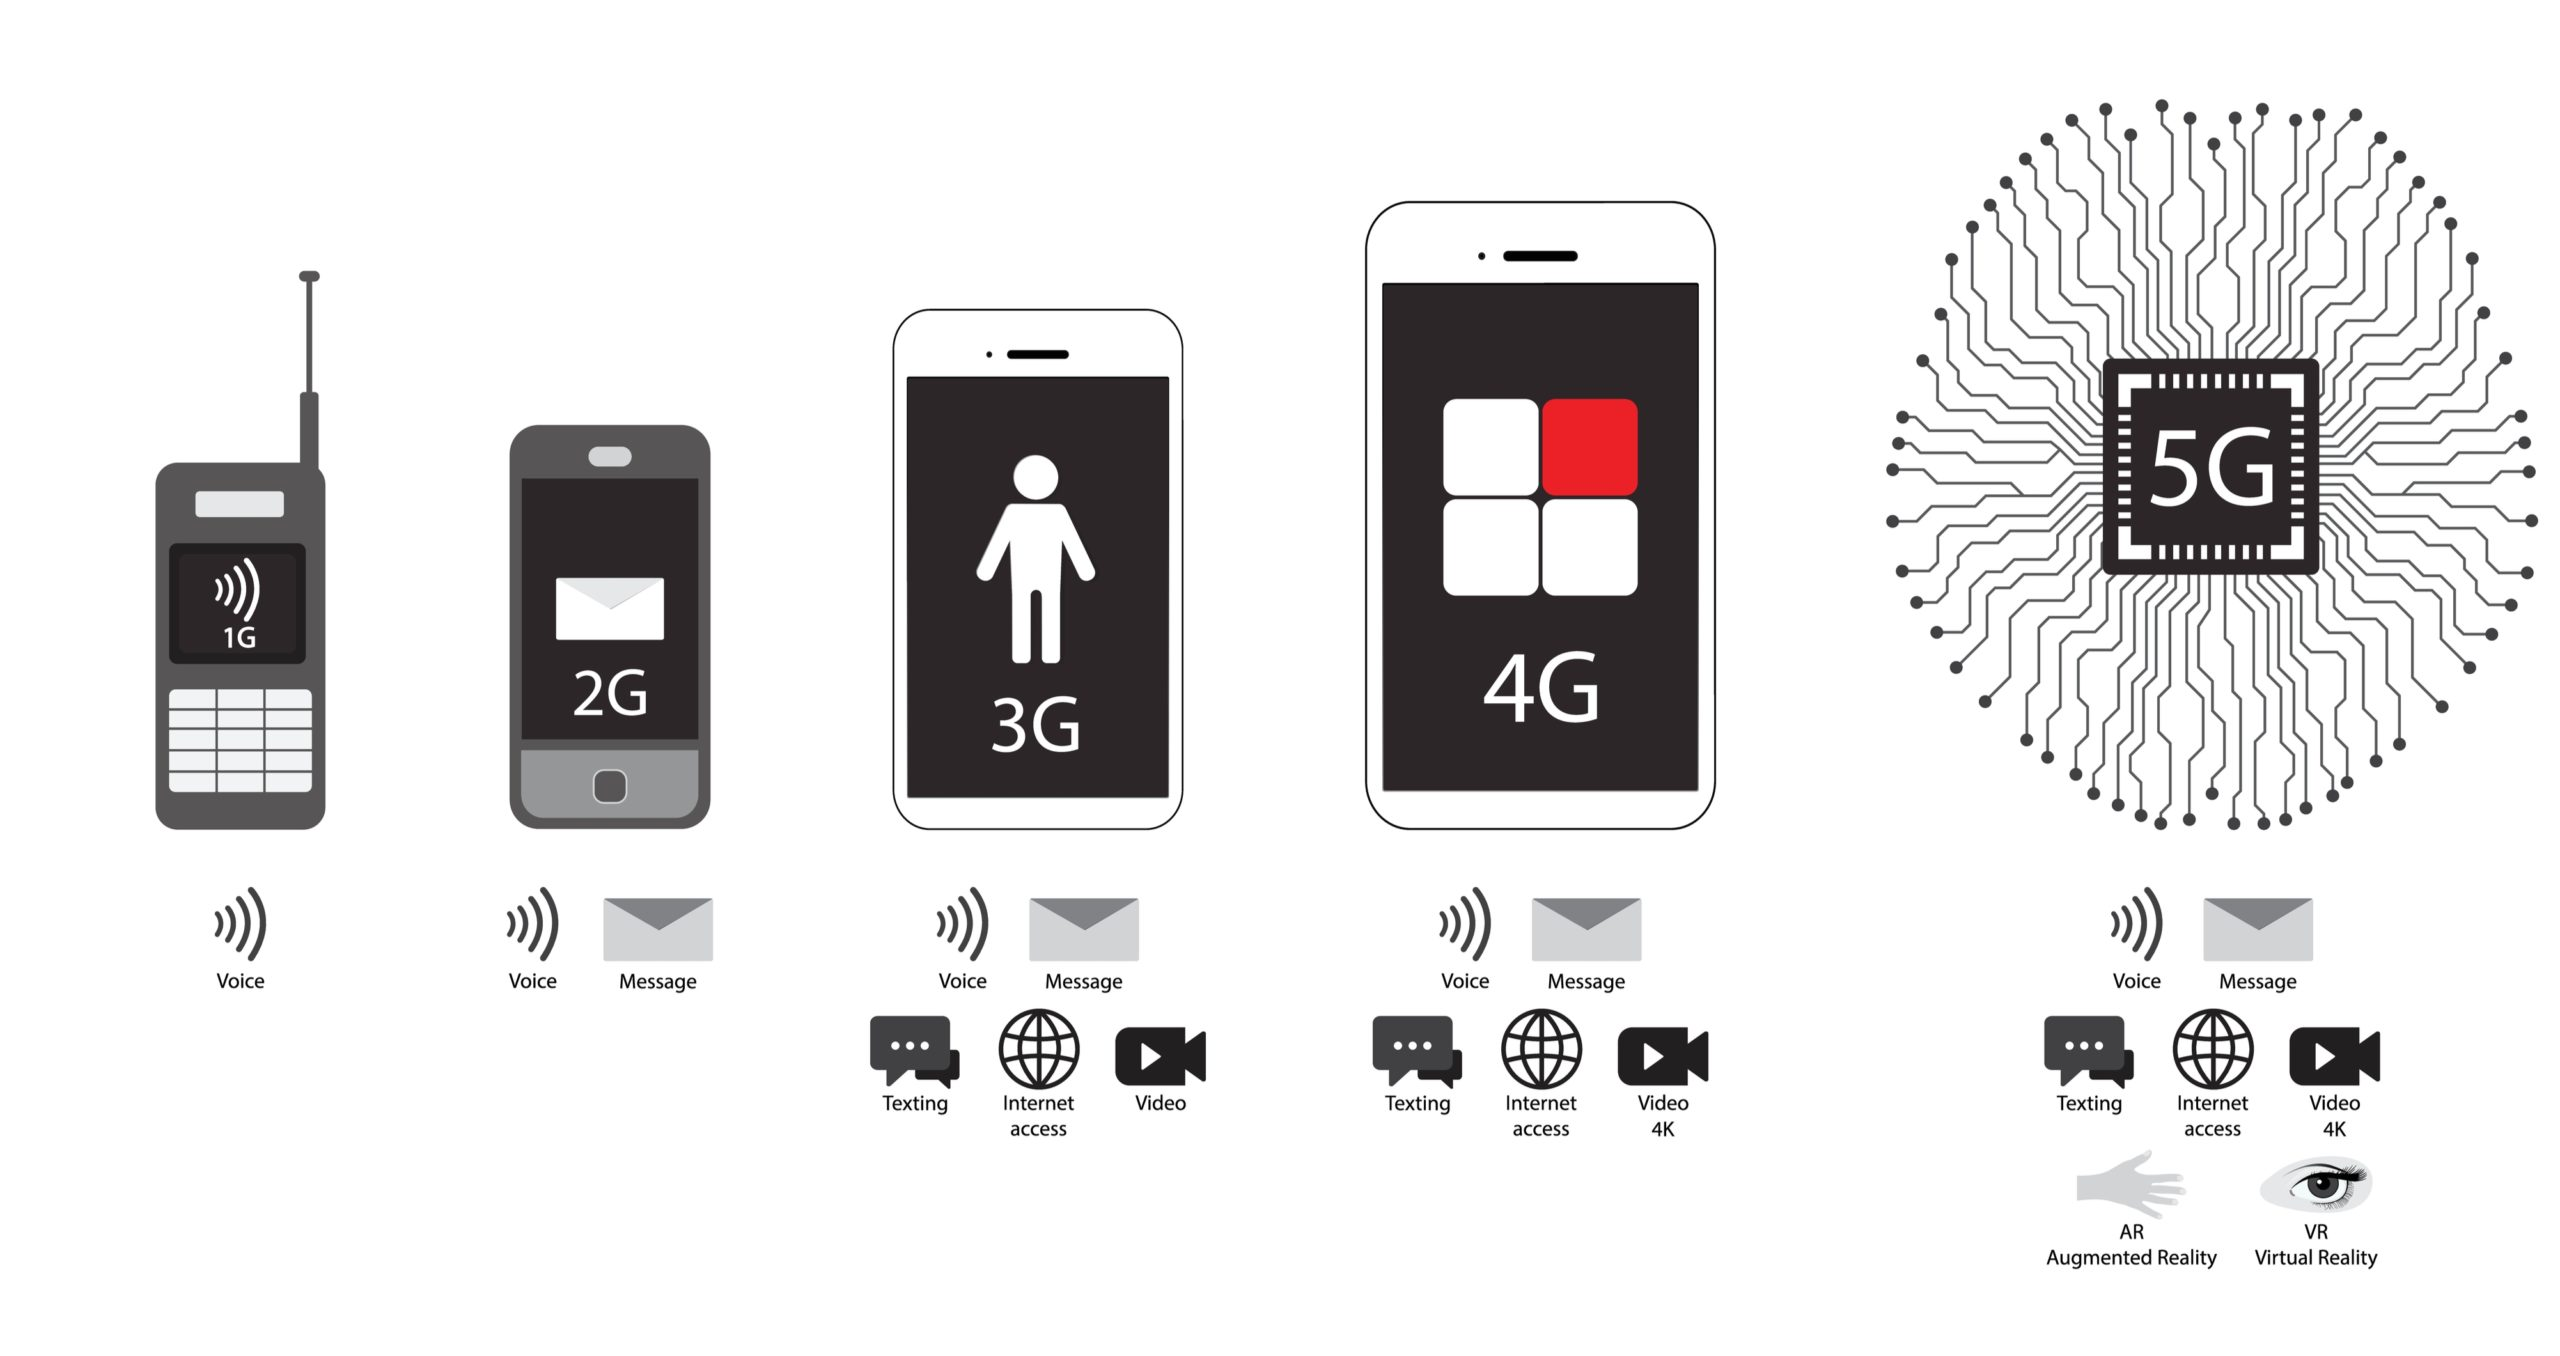
\includegraphics[width=0.7\textwidth]{images/generations-scheme.jpg}
    \caption{Schema delle generazioni cellulari}
\end{figure}

\subsection{1G}
La generazione 1G è uno dei primi standard di comunicazione cellulare. Il suo funzionamento era completamente analogico 
e ormai è stata rimpiazzata totalmente dalle generazioni digitali successive.\\
L'architettura di questa generazione è molto semplice, è composta da tre componenti principali:
\begin{itemize}
    \item Antenne per la trasmissione
    \item \textit{Mobile Telephone Switching Office} (MTSO)
    \item Unità mobile (cellulare)
\end{itemize}
\begin{figure}[ht]
    \centering
    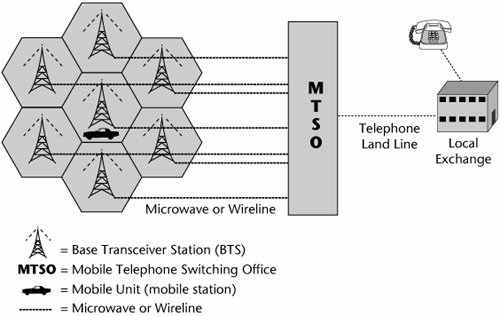
\includegraphics[width=0.7\textwidth]{images/1g.jpg}
    \caption{Architettura 1G}
\end{figure}
Si basava sulla \textit{frequency-division multiple access} (FDMA) in cui ogni dispositivo che si connetteva alla stazione radio
aveva assegnata una specifica sotto banda\cite{generations}.

\subsection{2G}
La seconda generazione cellulare è composta da diverse versioni che si sono susseguite nel corso degli anni aggiungendo nuove 
funzionalità.
La sua architettura verrà poi usata come base per le versioni successive.\\
Il MS si collega alla BTS di riferimento 
\begin{figure}[ht]
    \centering
    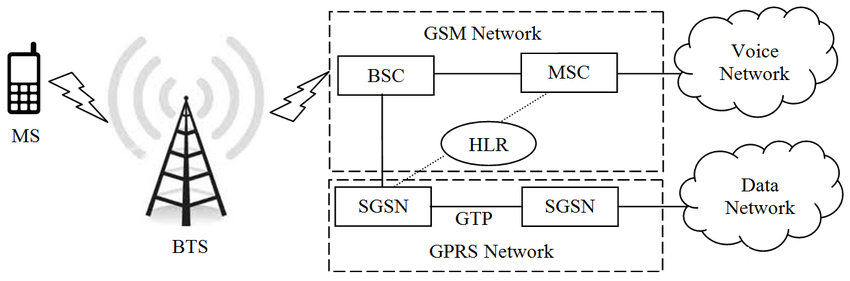
\includegraphics[width=0.7\textwidth]{images/2g-gsm-gprs.png}
    \caption{Architettura GSM e GPRS}
\end{figure}
\subsubsection{GSM}


\subsubsection{GPRS}


\subsubsection{EDGE}
Evoluzione del GPRS che consente maggiori velocità.

\subsection{3G}
\begin{figure}[ht]
    \centering
    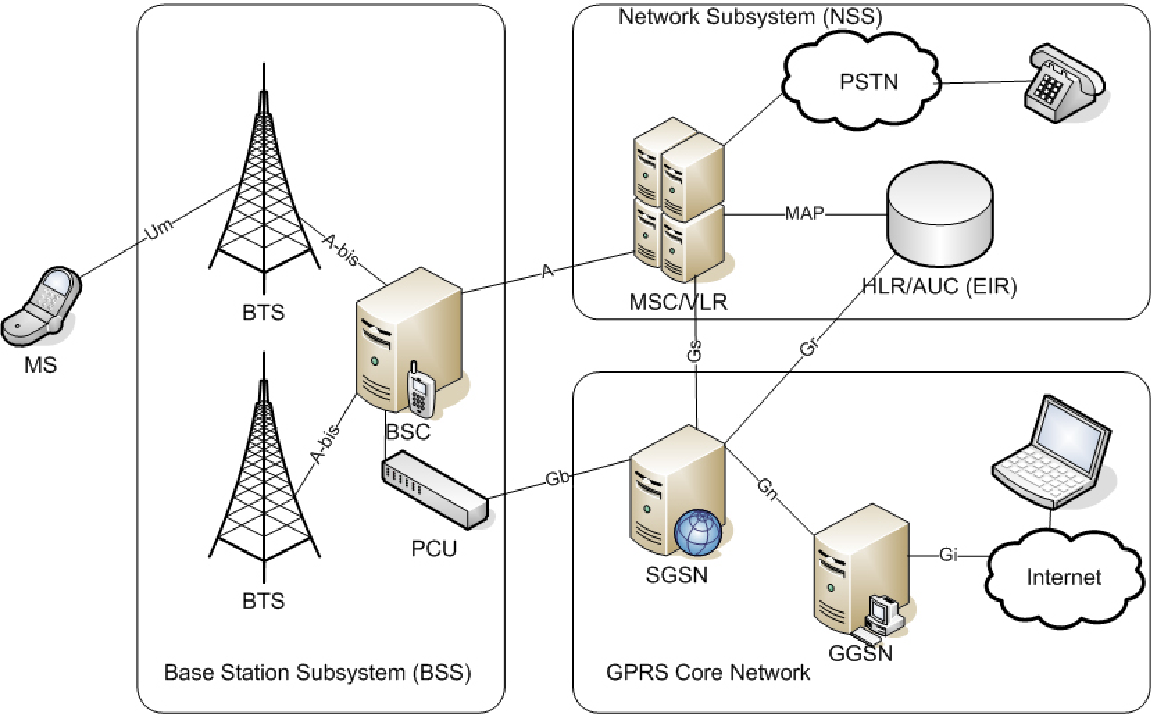
\includegraphics[width=0.7\textwidth]{images/3g-umts.png}
    \caption{Architettura UMTS}
\end{figure}

\subsubsection{UMTS}


\subsubsection{HSPA/HSPA+}


\subsection{4G}
\begin{figure}[ht]
    \centering
    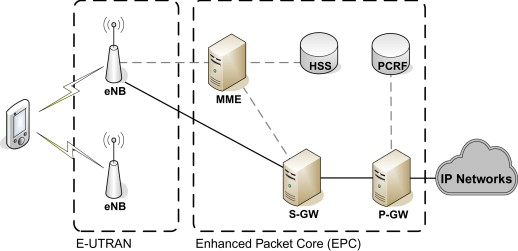
\includegraphics[width=0.8\textwidth]{images/4g-lte.jpg}
    \caption{Architettura LTE}
\end{figure}

\subsection{5G}
\begin{figure}[ht]
    \centering
    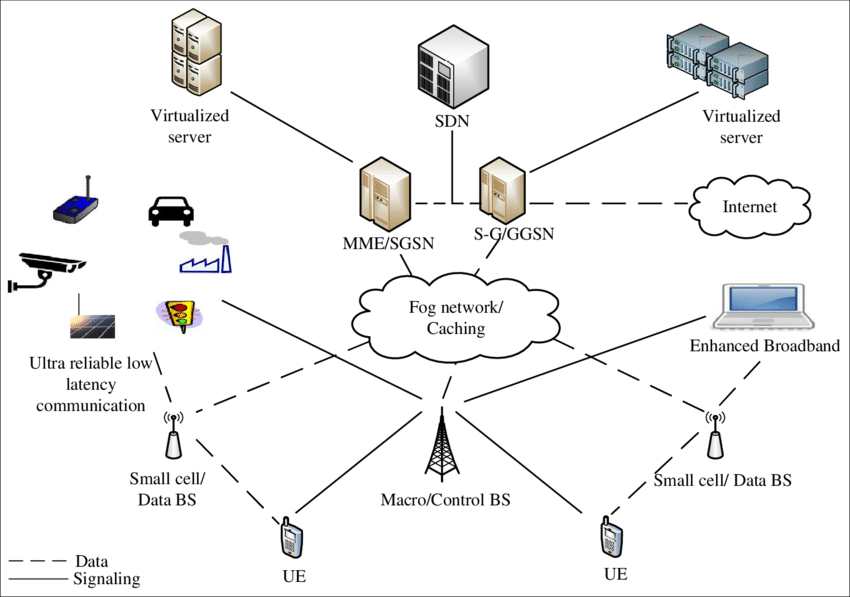
\includegraphics[width=0.7\textwidth]{images/5g.png}
    \caption{Architettura 5G}
\end{figure}